\setlength{\parskip}{\baselineskip}%
\setlength{\parindent}{0pt}%

In the winter of 1868/9, Swiss physician and biologist, Johannes Friedrich Miescher isolated an unknown substance from the nuclei of cells\cite{dahm2008discovering}. This substance was unlike anything he had observed before; it was resistant to protease, lacked sulphur and contained large amounts of phosphorous. He recognised that he had isolated a novel substance to which he named nuclein. Today, we know of this substance as deoxyribonucleic acid (DNA), the molecule of heredity.

Although Miescher speculated that nuclein may have had a role in hereditary, he later rejected the idea. It wasn't until 1944, when Oswald Avery, Colin MacLeod, and Maclyn McCarty were able to characterise the transforming factor in Griffith's Experiment\cite{griffith1928significance} as DNA\cite{avery1944studies}. They performed a series of biochemical experiments that isolated DNA and then demonstrated that by using an enzyme that only degraded DNA (deoxyribonucleodepolymerase or DNase), the transforming power was lost. It was later confirmed in 1952 by Alfred Hershey and Martha Chase that DNA is indeed the genetic material by the use of bacteriophages\cite{hershey1952independent}.

Fast forward to the 21st century and not only have we sequenced the entire collection of DNA of our very own species \cite{venter2001sequence, lander2001initial}, we can sequence an entire human genome in a matter of days by using high-throughput sequencers. We have also just recently reached the \$1,000 genome era, whereby we can sequence the entire genome of an individual for around \$1,000 US dollars. In contrast, the Human Genome Project, which gave us the first glimpse of the human genome costed around 2.7 billion in fiscal year 1991 US dollars\cite{nhgri2010cost}. This dramatic drop in sequencing cost means that DNA sequencing is much more accessible to scientists and medical practitioners who wish to apply sequencing to their work.

In the journal Nature Reviews Genetics, there is a stream of articles on the applications of high-throughput sequencing\cite{applicationsofsequencing}. These include, but are not limited to, studying gene expression, DNA-protein interactions, non-protein coding RNAs, DNA methylation, structural variants, histone modifications, DNA mutations, single-cells, and populations of bacteria. This thesis consists of several applications of DNA sequencing towards understanding a range of specific biological questions.

\section{The central dogma}

The molecular basis of heredity is DNA.

The relationship between genes and proteins 

\subsection{Transcription}

\subsection{RNA polymerase}

\subsection{Reverse transcription}

\section{DNA sequencing}

\subsection{Sanger / Maxam-Gilbert sequencing}

\subsection{Sequencing by synthesis}

\section{Applications of sequencing}

\section{Junk DNA}

Since the release of the draft human genome sequence\cite{lander2001initial}, it has been known that only a small fraction of the genome is made up of protein-coding sequences. The origin of the term "junk DNA" is usually attributed to Susumu Ohno, who used it to describe pseudogenes, which are non-functional gene copies. In its modern day usage, "junk DNA" is used to describe DNA sequence that goes not play a functional role in an organism. Dr. Ohno estimated that there would be an upper limit to the number of functional loci in mammalian genomes based on mutational load and a fixed mutation rate. He predicted that mammalian genomes could not have more than 30,000 loci under selection as this would guarantee a progressive decline in fitness, leading to extinction.

Talk about ENCODE here.

Blah blah blah.

\subsection{The repetitive genome}

\begin{figure}[h]
  \centering
  \includegraphics[width=10cm, angle=270]{barplot_repeat_family.eps}
  \caption[Tally of repetitive element families in the hg19 genome]
   {The number of repetitive element families determined by RepeatMasker in the hg19 genome.}
\end{figure}